\appendix

\section{Source Document Categories}
\label{app:sourcedocs}

\textbf{SEBI Documents:} SEBI (Issue of Capital and Disclosure Requirements) Regulations 2018, SEBI (Listing Obligations and Disclosure Requirements) Regulations 2015, SEBI (Substantial Acquisition of Shares and Takeovers) Regulations 2011, SEBI (Prohibition of Insider Trading) Regulations 2015, SEBI (Alternative Investment Funds) Regulations 2012, SEBI (Portfolio Managers) Regulations 2020, SEBI (Research Analysts) Regulations 2014, SEBI (Buy-Back of Securities) Regulations 2018, SEBI (Delisting of Equity Shares) Regulations 2021, SEBI (Mutual Funds) Regulations 1996, SEBI (Depositories and Participants) Regulations 2018, SEBI (Merchant Bankers) Regulations 1992, recent SEBI circulars (2024--2026).

\textbf{RBI Documents:} RBI Monetary Policy Statements (2024--2026), RBI Master Directions on Unique Identifiers in Financial Markets, RBI (Small Finance Banks---Prudential Norms on Declaration of Dividend) Directions 2026, Government Securities auction notifications (2025--2026), State Government securities auction press releases, RBI Weekly Statistical Supplement extracts, RBI circulars on KYC/AML compliance.

\section{System Prompt Template}
\label{app:prompt}

\begin{quote}
\noindent You are an expert in Indian financial regulation and policy. Answer questions using ONLY the provided context passage. Do not use any external knowledge. Be concise and precise. Give only the answer --- no preamble.
\end{quote}

\section{CON Task: Majority-Class Baseline and Balanced Accuracy}
\label{app:con}

The contradiction detection task (CON) has a class-imbalanced label distribution: 53 of 62 items (85.5\%) carry the gold label `No' (no contradiction exists), yielding a majority-class baseline accuracy of 85.5\%. Table~\ref{tab:c1} reports raw CON accuracy, margin over that baseline, and balanced accuracy (mean of sensitivity and specificity) computed from each model's per-item predictions. All models except Gemma 4 E4B and Mistral-7B exceed the majority-class baseline. Balanced accuracy preserves the raw-accuracy ordering; notably, most models detect the nine true contradictions perfectly (sensitivity 100\%) and differ mainly in false-positive rate on the 53 `No' items.

\begin{table}[t]
\centering\small
\begin{tabular}{lrrr}
\toprule
\textbf{Model} & \textbf{CON \%} & \textbf{vs. Base} & \textbf{Bal. Acc.} \\
\midrule
Gemini 2.5 Flash & 88.7 & +3.2 & 88.8 \\
Qwen3-32B & 90.3 & +4.8 & 94.3 \\
LLaMA-3.3-70B & 95.2 & +9.7 & 97.2 \\
Llama 4 Scout 17B & 98.4 & +12.9 & 99.1 \\
Kimi K2 & 91.9 & +6.4 & 95.3 \\
LLaMA-3-8B & 93.5 & +8.0 & 91.6 \\
GPT-OSS 120B & 95.2 & +9.7 & 97.2 \\
GPT-OSS 20B & 95.2 & +9.7 & 97.2 \\
Gemini 2.5 Pro & 93.5 & +8.0 & 91.6 \\
Mistral-7B & 80.6 & $-$4.9 & 88.7 \\
DeepSeek-R1-Distill-Llama-70B & 96.8 & +11.3 & 98.1 \\
Gemma 4 E4B & 79.0 & $-$6.5 & 87.7 \\
\midrule
Majority baseline & 85.5 & --- & 50.0 \\
\bottomrule
\end{tabular}
\caption{CON task raw accuracy, margin over the majority-class baseline (85.5\%), and balanced accuracy (mean of sensitivity and specificity over 9 `Yes' / 53 `No' gold labels).}
\label{tab:c1}
\end{table}

\section{Scoring Pipeline Validation}
\label{app:judge}

The automated scoring pipeline (Section~\ref{sec:scoring}) uses four stages: exact match, fuzzy token matching (RapidFuzz \texttt{token\_set\_ratio} $\geq$ 0.72), numerical extraction match, and Yes/No match for contradiction detection. While rigorous, the pipeline penalizes answers that are semantically correct but formatted differently from the reference answer---a systematic limitation of string-based matching for open-ended regulatory QA.

\subsection{Judge Rubric}

Both judges used in this paper---the Gemini 2.5 Flash pilot described below and the phi4-mini cross-model judge of Section~\ref{sec:judge}---were given the identical rubric, at temperature 0:

\begin{quote}\small\noindent
Determine if the model prediction is CORRECT.\\
Rules:\\
--- CORRECT if the final value or fact matches, even if: different formatting (currency symbols, comma separators, units), extra calculation steps shown before the final answer, paraphrasing of the same regulatory rule, or rounding within 1\%.\\
--- INCORRECT only if: wrong number, wrong threshold, wrong date, wrong entity, or contradicts the reference.\\
Reply with exactly: CORRECT or INCORRECT, plus a one-sentence reason.
\end{quote}

\subsection{Gemini Pilot}

Before committing to a full-coverage second judge, we piloted semantic re-scoring with Gemini 2.5 Flash---one of the twelve evaluated models---over items strict scoring marked incorrect across NUM, REG, and TMP. The strict pipeline flagged 935 such predictions; 874 were judged, and the remaining 61 (58 empty responses, 3 API failures) were retained as incorrect without review, since no semantic judgment can rescue an empty prediction. CON items use exact Yes/No matching and were not part of this pilot.

Judge reliability was estimated on a stratified 28-item manual audit (20 NUM, 5 REG, 3 TMP). Manual review confirmed 25 of 28 verdicts (89.3\%) as correct. The three judge errors all involved multi-step numerical problems where the model showed correct intermediate reasoning but reached a wrong final answer (NUM\_074: predicted Rs.~19,000 crore vs.\ reference Rs.~33,000 crore; NUM\_103: concluded wrong direction for a threshold comparison; NUM\_136: applied wrong regulatory fee slab)---the judge's tendency to over-credit partial reasoning chains on NUM items, referenced in Section~\ref{sec:discussion}. Across the 874 judged predictions, Gemini reclassified 685 from incorrect to correct, an overall flip rate of 78.4\% (REG: 261/327 = 79.8\%; NUM: 272/348 = 78.2\%; TMP: 152/199 = 76.4\%).

Because Gemini is itself one of the evaluated models and this pilot covered only strict failures---so it could characterise strict-to-judge overturns but not the judge's rejection rate of strict-correct predictions---these results motivated, rather than substitute for, the full-coverage cross-model judge (phi4-mini, sharing no model family with any evaluated system, reviewing all 4{,}128 REG/NUM/TMP predictions including strict-correct ones) whose results are reported in Section~\ref{sec:judge} and Table~\ref{tab:judgereliability}. Item-level Gemini verdicts remain available at \texttt{evaluation/results\_judged/} in the repository; the final judge-audited accuracies used throughout this paper are computed from phi4-mini's full-coverage pass (\texttt{evaluation/results\_judged\_phi4/}), not from this pilot.

\subsection{Root Causes}

Three systematic causes, identified during the Gemini pilot and consistent with the phi4-mini overturn cases, account for the majority of strict-to-judge overturns: (1) \textit{Numeric format differences} --- models frequently use digits (`50\%', `365 days') while references use written numbers (`fifty per cent', `three hundred and sixty-five days'). (2) \textit{Verbose answers} --- models prefix the correct answer with calculation steps or regulatory citations. (3) \textit{Abbreviated answers} --- models give a shorter but correct version of the reference (e.g., ref = `Six months after completion of the open offer'; pred = `Six months').

\subsection{Human Adjudication Protocol}

To check both judges against a human reader, we built a 238-item adjudication sheet (\texttt{annotation/judge\_audit/adjudication\_sheet.csv}, \texttt{scripts/build\_adjudication\_control\_sample.py}): the 174 REG/NUM/TMP items where Gemini and phi4-mini disagree---the only cases informative about which judge is right---plus a stratified control sample of 64 items (8 per stratum, fixed random seed) spanning cases where the available methods \emph{agree}: \texttt{\{REG,NUM,TMP\}\_strict\_incorrect\_judges\_agree} (both judges concur an item is wrong), \texttt{\{REG,NUM,TMP\}\_strict\_correct\_phi4\_agrees} (phi4-mini does not dispute a strict-correct item; no Gemini verdict exists for these, since Gemini only ever judged strict failures), and two CON strata (\texttt{CON\_strict\_correct\_no\_judge}, \texttt{CON\_strict\_incorrect\_no\_judge}) that spot-check the exact-match scorer directly, since CON is never judge-reviewed by either model. This sample is evidence about specific, informative cases, not a random draw sized to estimate a population-level judge error rate, and Section~\ref{sec:judge} reports it as such.

\subsection{Human Adjudication Results}

All 238 items were adjudicated by the author. Section~\ref{sec:judge} reports the headline split (89.1\% control-agreement, 56.9\%/43.1\% Gemini/phi4-mini on disputed items); per stratum, the control-agreement rate ranged from 75.0\% (\texttt{NUM\_strict\_incorrect\_judges\_agree}, \texttt{TMP\_strict\_correct\_phi4\_agrees}) to 100\% (both CON strata and \texttt{REG\_strict\_correct\_phi4\_agrees}), with no stratum below 75\%---agreement between methods tracked human judgment reasonably well across every category sampled, not only on average. Section~\ref{sec:limitations} reports the DeepSeek-R1-Distill-specific breakdown of the disputed-item sample.

\section{Evaluated Models}
\label{app:models}

\begin{table}[t]
\centering\footnotesize
\begin{tabular}{lp{2.4cm}p{1.5cm}}
\toprule
\textbf{Model} & \textbf{Provider / Access} & \textbf{Params} \\
\midrule
Gemini 2.5 Flash & Google (AI Studio API) & --- \\
Gemini 2.5 Pro & Google (Vertex AI) & --- \\
Qwen3-32B & Alibaba (Groq API) & 32B \\
LLaMA-3.3-70B & Meta (Groq API) & 70B \\
Llama 4 Scout 17B & Meta (Groq API) & 17B \\
Kimi K2 & Moonshot AI (Groq API) & 1T total, 32B active (MoE) \\
LLaMA-3-8B & Meta (Ollama, local) & 8B \\
GPT-OSS 120B\textdaggerdbl{} & OpenAI (open-weight, Groq API) & 120B \\
GPT-OSS 20B\textdaggerdbl{} & OpenAI (open-weight, Groq API) & 20B \\
Mistral-7B & Mistral AI (Ollama, local) & 7B \\
DeepSeek-R1-Distill-Llama-70B & DeepSeek (Groq API) & 70B \\
Gemma 4 E4B & Google (Ollama, local) & 4B \\
\bottomrule
\end{tabular}
\caption{Models evaluated in this study. \textdaggerdbl{}OpenAI open-weight models accessed via the Groq inference API. Local models ran on an Intel i7-13650HX CPU with an NVIDIA RTX 4060 GPU (8~GB VRAM); exact identifiers were \texttt{llama3:8b}, \texttt{mistral:7b}, and \texttt{gemma3:4b}, with temperature 0.0 via the Ollama REST API.}
\label{tab:models}
\end{table}

\section{Task Examples, Pipeline, and Failure Cases}
\label{app:examples}

Figure~\ref{fig:pipeline} illustrates the dataset construction pipeline. Figure~\ref{fig:taskexamples} shows a representative item for each task type; Figure~\ref{fig:heatmap} visualizes per-task accuracy across all twelve models.

\begin{figure*}[t]
\centering
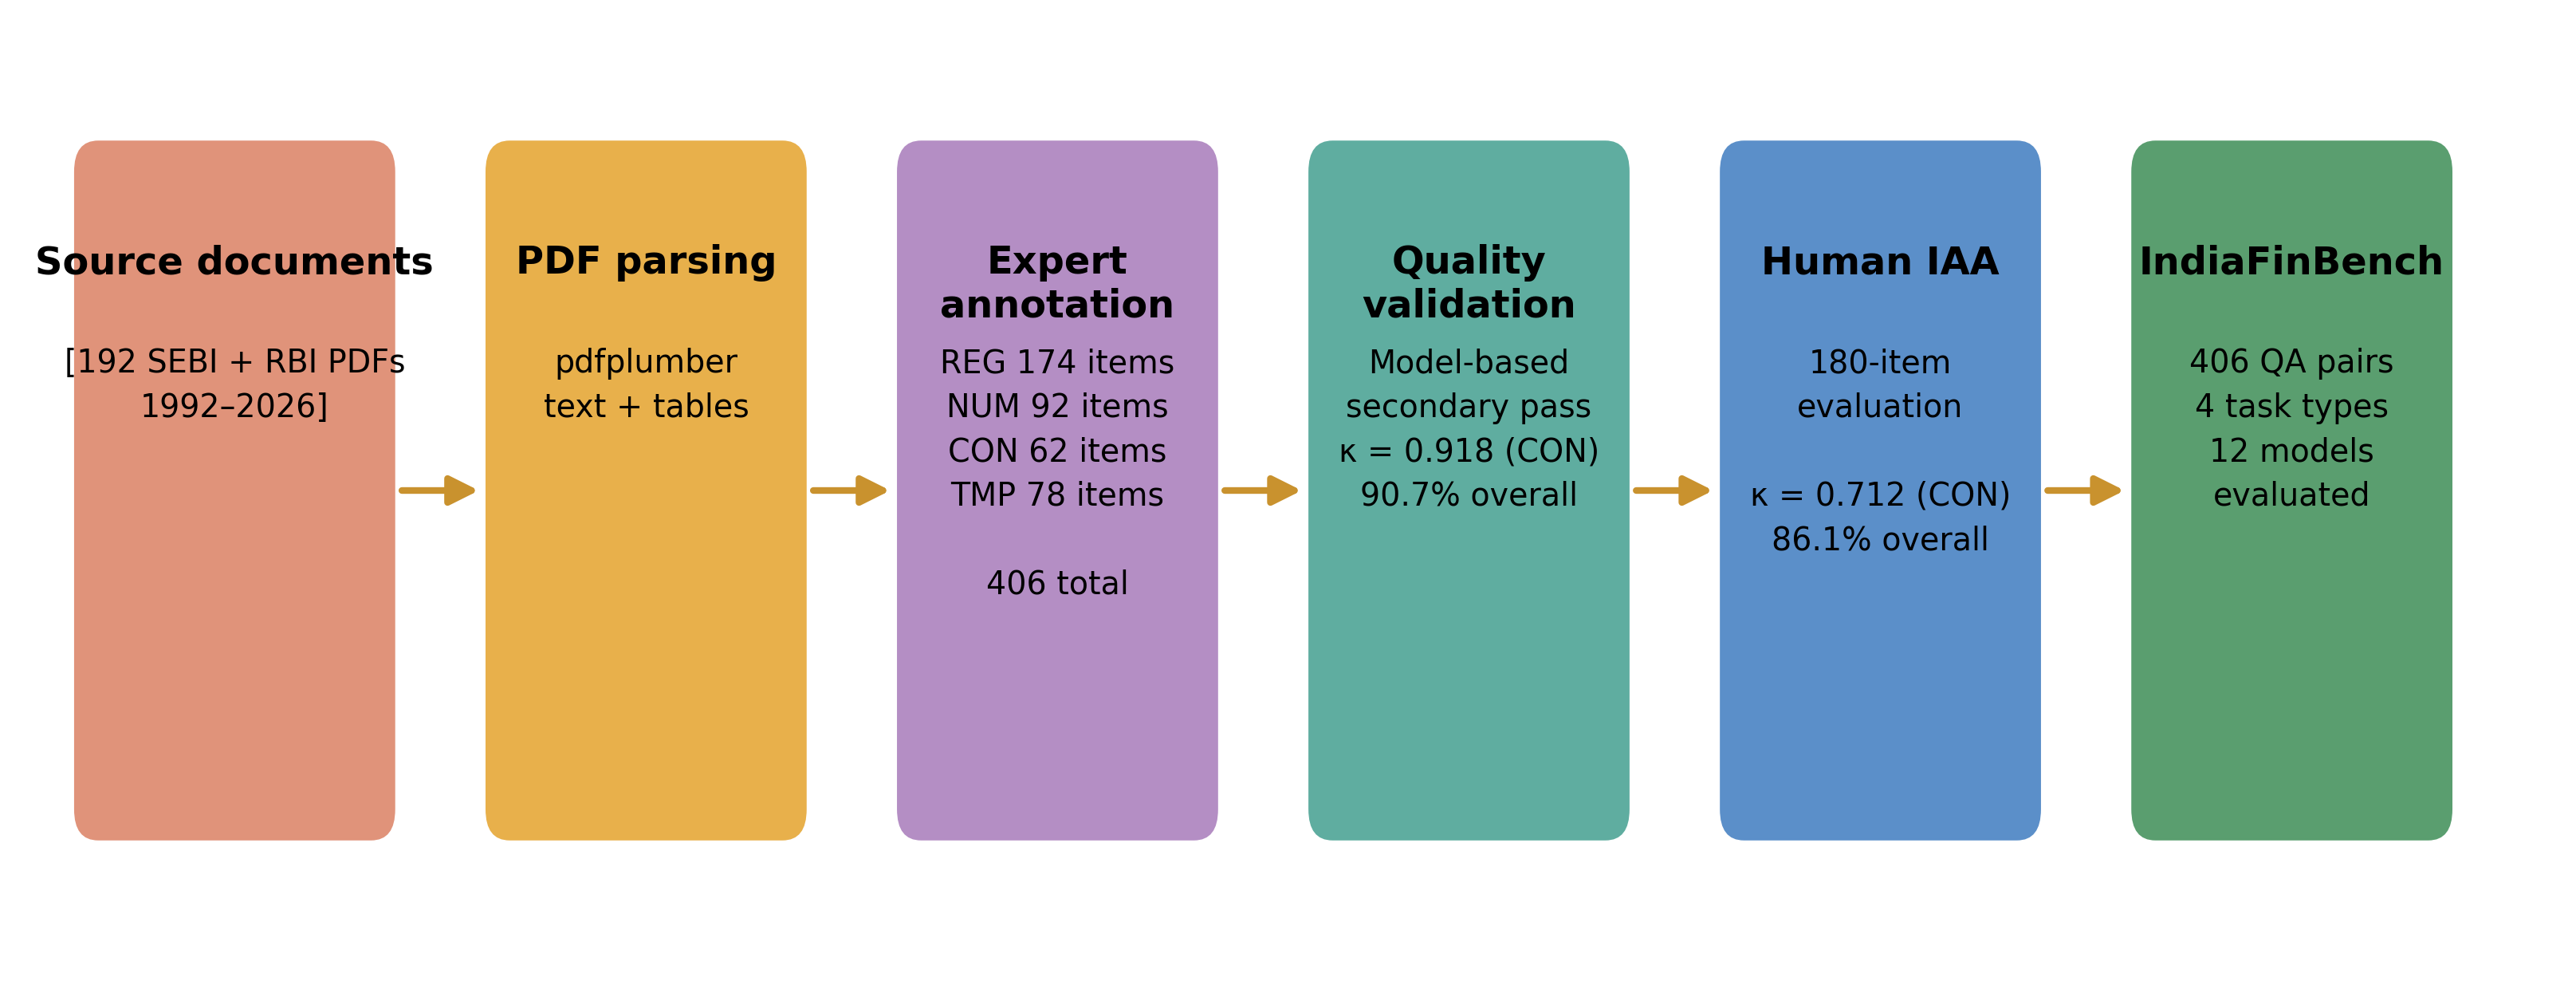
\includegraphics[width=0.85\textwidth]{figures/fig_pipeline.png}
\caption{IndiaFinBench dataset construction pipeline. Starting from 192 SEBI and RBI PDFs (1992--2026), documents are parsed using pdfplumber and expert-annotated into 406 QA items across four task types (REG: 174, NUM: 92, CON: 62, TMP: 78). Quality is validated through a model-based secondary pass ($\kappa$ = 0.918 on CON; 90.7\% overall) and a 180-item human inter-annotator agreement study ($\kappa$ = 0.645 on CON; 77.2\% overall), yielding a benchmark evaluated on 12 models under zero-shot conditions.}
\label{fig:pipeline}
\end{figure*}

\begin{figure*}[t]
\centering

\includegraphics[width=0.85\textwidth]{figures/fig_taskexamples.png}
\caption{Representative examples of all four IndiaFinBench task types. REG (regulatory interpretation): the model extracts the correct compliance deadline from a SEBI passage. NUM (numerical reasoning): the model computes the maximum dividend payout for a Small Finance Bank using RBI Dividend Directions 2026, requiring multi-step arithmetic. CON (contradiction detection): the model determines whether two regulatory passages conflict, identifying that a surface-level phrasing difference (written numeral vs. digit) does not constitute a substantive contradiction. TMP (temporal reasoning): the model identifies the operative version of SEBI Insider Trading Regulations at a specific historical date. Reference answers are underlined.}
\label{fig:taskexamples}
\end{figure*}

\begin{figure}[t]
\centering

\includegraphics[width=\columnwidth]{figures/fig_heatmap.png}
\caption{Performance heatmap across all twelve models and four task types under strict scoring. Darker cells indicate higher accuracy.}
\label{fig:heatmap}
\end{figure}

\paragraph{Representative failure examples.}

\textbf{Domain Knowledge Failure (Gemma 4 E4B, Temporal Reasoning, item TMP\_039).} Asked whether a December~15, 2026 OTC derivative transaction is subject to Unique Transaction Identifier requirements that take effect January~1, 2027, the model answers ``Yes,'' misapplying the forward-looking effective date to a transaction entered into before it; the reference answer is ``No,'' since the requirements do not yet apply. (Hard temporal-reasoning items map to DKF under the taxonomy of Appendix~\ref{sec:errortax-sub}, since the failure is a substantive misunderstanding of when a rule takes effect, not a surface mismatch.)

\textbf{Numerical Reasoning Failure (GPT-OSS 120B, Numerical Reasoning).} Given an RBI calculation requiring the maximum eligible dividend as a percentage of adjusted PAT, the model correctly identifies the relevant table but applies the wrong conditional threshold, computing the dividend at a higher rate than is warranted by the given capital ratio.

\textbf{Temporal Reasoning Failure (DeepSeek-R1-Distill-Llama-70B, Temporal Reasoning, item TMP\_036).} Asked when the SEBI (Research Analysts) Regulations 2014---published September~1, 2014, effective ninety days later---came into force, the model answers ``November 29, 2014''; the reference date is November 30, 2014, one day later. The model's day-count method is correct; its arithmetic is off by one day.

\textbf{Context Grounding Failure (LLaMA-3.3-70B, Contradiction Detection).} Given two RBI passages specifying the same 5\% non-competitive bidding allocation limit in different phrasing (`five per cent' vs.\ `5\%'), the model incorrectly identifies a contradiction based on surface-level differences rather than recognizing semantic equivalence.

\section{Difficulty Breakdown and Task Profiles}
\label{app:difficulty}

Table~\ref{tab:difficulty} reports per-model accuracy by difficulty level; Figure~\ref{fig:difficulty} plots the trajectories, Figure~\ref{fig:radar} shows per-task accuracy profiles, and Figure~\ref{fig:correlation} gives the inter-task correlation structure.

\begin{figure}[t]
\centering

\includegraphics[width=\columnwidth]{figures/fig_correlation.png}
\caption{Inter-task correlation matrix across the four task types. Values indicate Spearman $\rho$ correlation of per-model accuracy vectors across tasks (n=12 models). With n=12, the critical $\rho$ for significance at p$<$0.05 (two-tailed) is approximately 0.58; no pairwise inter-task correlation reaches this threshold: NUM--TMP is the largest at $\rho$=0.50, REG--CON and NUM--CON are weakly negative ($\rho\approx-0.33$), and the remaining pairs are small and positive. Task performance is largely task-specific rather than reflecting one latent capability.}
\label{fig:correlation}
\end{figure}

\begin{table}[t]
\centering\footnotesize
\begin{tabular}{lrrr}
\toprule
\textbf{Model} & \textbf{Easy} & \textbf{Med.} & \textbf{Hard} \\
 & \textit{(n=160)} & \textit{(n=182)} & \textit{(n=64)} \\
\midrule
Gemini 2.5 Flash & 92.5 & 89.0 & 84.4 \\
Qwen3-32B & 81.9 & 87.9 & 87.5 \\
LLaMA-3.3-70B & 79.4 & 85.2 & 90.6 \\
Llama 4 Scout 17B & 82.5 & 81.9 & 89.1 \\
Kimi K2 & 81.9 & 80.8 & 82.8 \\
LLaMA-3-8B & 76.2 & 79.7 & 78.1 \\
GPT-OSS 120B & 79.4 & 76.4 & 73.4 \\
GPT-OSS 20B & 75.0 & 79.7 & 73.4 \\
Gemini 2.5 Pro\textdagger{} & 83.1 & 72.5 & 68.8 \\
Mistral-7B & 74.4 & 76.9 & 76.6 \\
DeepSeek-R1-Distill-Llama-70B & 72.5 & 77.5 & 75.0 \\
Gemma 4 E4B & 82.5 & 74.7 & 81.2 \\
\bottomrule
\end{tabular}
\caption{Accuracy (\%) by difficulty level (full 406-item evaluation, strict pipeline). \textdagger{}Verbose-output scoring artifact; see Appendix~\ref{app:judge}.}
\label{tab:difficulty}
\end{table}

\begin{figure*}[t]
\centering

\includegraphics[width=0.75\textwidth]{figures/fig_difficulty.png}
\caption{Per-model accuracy across difficulty levels (Easy / Medium / Hard). Lines connect the three difficulty conditions for each model.}
\label{fig:difficulty}
\end{figure*}

\begin{figure}[t]
\centering

\includegraphics[width=\columnwidth]{figures/fig_radar.png}
\caption{Radar chart comparing per-task accuracy profiles across models. Each axis represents a task type.}
\label{fig:radar}
\end{figure}

\section{Few-Shot Evaluation}
\label{app:fewshot}

To assess whether zero-shot evaluation represents a conservative lower bound on model capability, we evaluated four top-performing models---Gemini 2.5 Flash, LLaMA-3.3-70B, Llama 4 Scout 17B, and Qwen3-32B---under 3-shot prompting. For each task type, three fixed in-context examples were prepended to the prompt, drawn from the same distribution as the benchmark items and held constant across all models. All other evaluation conditions (system prompt, scoring pipeline, dataset) were identical to the zero-shot setup.

\begin{table*}[t]
\centering\small
\begin{tabular}{llrrrrr}
\toprule
\textbf{Model} & \textbf{Cond.} & \textbf{REG} & \textbf{NUM} & \textbf{CON} & \textbf{TMP} & \textbf{Overall} \\
\midrule
\multirow{3}{*}{Gemini 2.5 Flash} & 0-shot & 93.1\% & 84.8\% & 88.7\% & 88.5\% & 89.7\% \\
 & 3-shot & 92.0\% & 87.0\% & 91.9\% & 88.5\% & 90.1\% \\
 & $\Delta$ & $-$1.1 & +2.2 & +3.2 & +0.0 & +0.4 \\
\midrule
\multirow{3}{*}{Qwen3-32B} & 0-shot & 85.1\% & 77.2\% & 90.3\% & 92.3\% & 85.5\% \\
 & 3-shot & 86.8\% & 79.3\% & 90.3\% & 92.3\% & 86.7\% \\
 & $\Delta$ & +1.7 & +2.1 & +0.0 & +0.0 & +1.2 \\
\midrule
\multirow{3}{*}{LLaMA-3.3-70B} & 0-shot & 86.2\% & 75.0\% & 95.2\% & 79.5\% & 83.7\% \\
 & 3-shot & 87.4\% & 77.2\% & 98.4\% & 87.2\% & 86.7\% \\
 & $\Delta$ & +1.2 & +2.2 & +3.2 & +7.7 & +3.0 \\
\midrule
\multirow{3}{*}{Llama 4 Scout 17B} & 0-shot & 86.2\% & 66.3\% & 98.4\% & 84.6\% & 83.3\% \\
 & 3-shot & 90.2\% & 82.6\% & 85.5\% & 76.9\% & 85.2\% \\
 & $\Delta$ & +4.0 & +16.3 & $-$12.9 & $-$7.7 & +1.9 \\
\bottomrule
\end{tabular}
\caption{Zero-shot vs. 3-shot accuracy by task type.}
\label{tab:e1}
\end{table*}

3-shot prompting improves numerical reasoning by 2.1--16.3 percentage points across all four models, with Llama 4 Scout 17B showing the largest NUM gain (+16.3 pp, from 66.3\% to 82.6\%). LLaMA-3.3-70B gains +7.7 pp on temporal reasoning under 3-shot. These improvements confirm the direction of the zero-shot conservatism claimed in Section~\ref{sec:main-results-text} without altering comparative structure.

CON performance is mixed: Llama 4 Scout 17B declines 12.9 pp (from near-ceiling 98.4\% to 85.5\%), while Gemini 2.5 Flash improves +3.2 pp. Performance degradation under 3-shot on tasks with near-ceiling zero-shot accuracy is consistent with in-context example interference, where the few-shot prefix biases the model away from clear Yes/No responses on straightforward contradiction items. Qwen3-32B is unaffected on CON and TMP (0.0 pp), suggesting its zero-shot behavior is already well-calibrated for these task types.

Overall, the performance tier ordering is preserved under 3-shot prompting (Gemini 2.5 Flash $\geq$ Qwen3-32B $\geq$ LLaMA-3.3-70B $\approx$ Llama 4 Scout 17B), confirming that the tier structure observed in zero-shot evaluation reflects genuine model capability differences rather than prompting strategy sensitivity.

\end{document}
